\documentclass[tikz,border=10pt]{standalone}
% No extra libraries needed for this figure.
\begin{document}
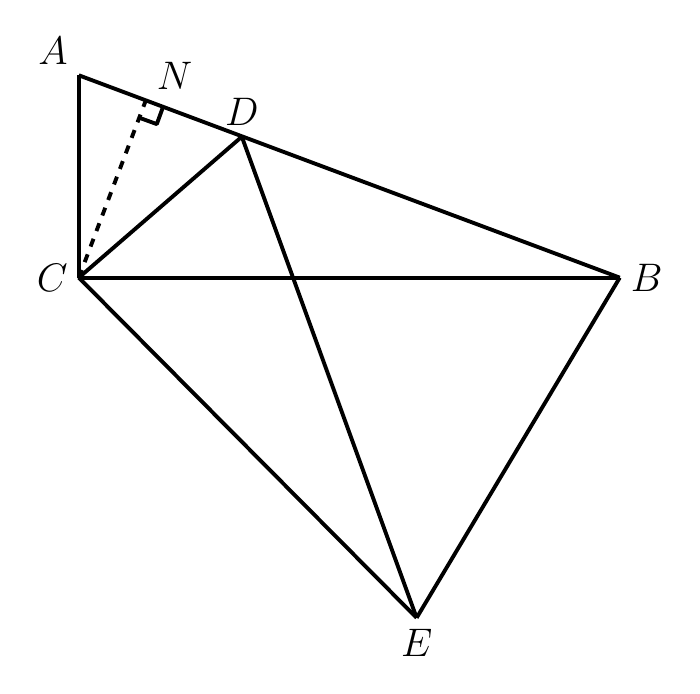
\begin{tikzpicture}[line join=round, line width=1.4pt]
  % Coordinates: scale s = 0.018223 cm/px, centred on ink bbox (cx=245, cy=225), y flipped
  \coordinate (A) at (-3.48,3.48);
  \coordinate (N) at (-2.63,3.16);
  \coordinate (D) at (-1.41,2.70);
  \coordinate (B) at (3.39,0.91);
  \coordinate (C) at (-3.48,0.91);
  \coordinate (E) at (0.81,-3.41);

  % Main solid segments
  \draw (A) -- (B);   % line AB (contains D and N)
  \draw (A) -- (C);   % vertical AC
  \draw (C) -- (B);   % horizontal CB
  \draw (C) -- (E);
  \draw (D) -- (E);
  \draw (B) -- (E);
  \draw (C) -- (D);

  % Dashed altitude CN
  \draw[dashed] (C) -- (N);

  % Right-angle mark at N (from mark_points_px converted to cm)
  \draw (-2.41,3.08) -- (-2.49,2.86) -- (-2.71,2.94);

  % Labels
  \node[above left] at (A) {\fontsize{14.5}{17.4}\selectfont $A$};
  \node[above right] at (N) {\fontsize{14.5}{17.4}\selectfont $N$};
  \node[above] at (D) {\fontsize{14.5}{17.4}\selectfont $D$};
  \node[right] at (B) {\fontsize{14.5}{17.4}\selectfont $B$};
  \node[left] at (C) {\fontsize{14.5}{17.4}\selectfont $C$};
  \node[below] at (E) {\fontsize{14.5}{17.4}\selectfont $E$};
\end{tikzpicture}
\end{document}